\documentclass[10pt]{article}
\usepackage[total={170mm,230mm}]{geometry}

\usepackage{cmap}
\usepackage[utf8]{inputenc}
\usepackage[T2A]{fontenc}
\usepackage[russian]{babel}
\usepackage{hyphsubst}

\usepackage{graphicx}
\usepackage{xcolor}
\usepackage{amssymb}
\usepackage{amsfonts}
\usepackage{amsmath}
\usepackage{amsthm}
\usepackage{physics}
\usepackage{wrapfig}
\usepackage{cancel}
\usepackage{pdfpages}
\usepackage{hyperref}
\usepackage{caption}
\usepackage{subcaption}
% \usepackage{bibtex}

\title{Домашнее задание №6. Динамика гауссовского волнового пакета на фиксированном промежутке с использованием маскирующей функции}
\author{Александр Козлов}
\date{\today}

\begin{document}

\maketitle

\section*{Формулировка задания}

Рассматривается временное уравение Шрёдингера $i \partial_t \Psi = H \Psi$ с начальным условием $$\Psi(k,t=0) = \exp(-(k-k_0)^2),$$ где $k$ --- волновое число (в атомных единицах --- в которых, мы, собственно, и работаем --- тождественно импульсу). Необходимо воспроизвести свбодную (то есть $H=-\laplacian$ в атомарных единицах) динамику гауссовского волнового пакета на фиксированном промежутке с использованием маскирующей функции $M(x)$ и сравнить численное решение с аналитическим.

\section{Решения задачи с использованием маскировочной функции}

\subsection*{Сетка}
Прежде всего зададим равномерную сетку
\begin{equation}
	x_0 = -R,\; x_1 = x_0 + \delta,\; x_2 = x_0 + 2\delta,\; \ldots,\; x_k = x_0 + k\delta,\; \ldots,\; x_M = x_0 + M \delta = R
\end{equation}
с шагом $\delta = 2R/M$, где $M$~---~целое положительное число, а $R$~---~положительное действительное число.

\subsection*{Маскировочная функция}
В качестве маскировочной функции возьмём такую:
\begin{equation}
	M(x) = \exp\qty[-\qty(\dfrac{x}{R-\delta_M})^{10}].
% 	\begin{cases}
% 		-\dfrac{2}{\delta_M^3}(x+R-\delta_M)^3 - \dfrac{3}{\delta_M^2} (x+R-\delta_M)^2 + 1, &x\in(-R,\; -R+\delta_M);\\
% 		1, &x\in(-R+\delta_M,\; R-\delta_M);\\
% 		\dfrac{2}{\delta_M^3}(x-R+\delta_M)^3 - \dfrac{3}{\delta_M^2} (x-R+\delta_M)^2 + 1, &x\in(R-\delta_M,\; R)
% 	\end{cases}
\end{equation}

\subsection*{Аналитическое решение}

В начальный момент времени $t=0$ волновая функция в импульсном пространстве имеет вид $$\Psi(k,t=0) = \exp(-(k-k_0)^2),$$ где $k$ --- волновое число (в атомных единицах --- в которых мы работаем --- тождественно импульсу). Гамильтониан свободного пространства в импульсном пространстве имеет вид $$ \mathrm{H} = k^2,$$ поэтому решение времянного УШ в импульсном пространстве легко написать. Оно будет иметь вид:
\begin{equation}
 \Psi(k,t) =\exp\qty(-i k^2 t - (k-k_0)^2).
\end{equation}
В прострвенных координатах $x$ такая волновая функция будет иметь вид:
\begin{equation}
 \Psi(x,t) =  C \cdot \int \dd{k} \exp\qty(ikx -i k^2 t - (k-k_0)^2) = C \cdot \sqrt{\dfrac{\pi}{it+1}} \exp\qty(\dfrac{(2k_0 + ix)^2}{4(it+1)} - k_0^2),
\end{equation}
где $C$ --- некоторый нормировочный множитель. Выберем $C$ таким образом, чтобы $\norm{\Psi(x,t=0)}^2=1$. Тогда $C=(2\pi^3)^{-1/4}$ и аналитическое решение имеет вид:
\begin{equation}
 \Psi(x,t) = \sqrt[4]{\dfrac{1}{2\pi}} \sqrt{\dfrac{1}{it+1}} \exp\qty(\dfrac{(2k_0 + ix)^2}{4(it+1)} - k_0^2).
\end{equation}

\subsection*{Итерационная последовательность волновых функций}
Для решения задачи строим итерационную последовательность волновых функций, обозначать которые будем через $\Psi^{(M)}_n(x\in[-R,\,R])$, где $n$ --- номер шага по времени. Волновая функция $\Psi^{(M)}_n(x)$, полученная предложенным алгоритмом решения, является приближением точного решения $\Psi(x,\, t=n\tau)$, где $\tau$ --- шаг по времени. Последовательность функций $\qty{\Psi^{(M)}_n(x)}_{n=0}^{N}$ формируется следующим образом:
\begin{equation}
	\begin{split}
		\Psi^{(M)}_0(x) &= M(x)\, \Psi(x,t=0),\\
		\Psi^{(M)}_1(x) &= M(x)\, e^{-i H \tau} \Psi^{(M)}_0(x),\\
		&\ldots\\
		\Psi^{(M)}_n(x) &= M(x)\, e^{-i H \tau} \Psi^{(M)}_{n-1}(x),\\
		&\ldots\\
		\Psi^{(M)}_N(x) &= M(x)\, e^{-i H \tau} \Psi^{(M)}_{N-1}(x).
	\end{split}
\end{equation}

Оператор эволюции $e^{-i H \tau}$, выбрав шаг по времени достаточно малым, можно расчитывать используя Паде-апрроксимацию.

\section{Результаты и сопоставление численного решения с аналитическим}

На Рис. \ref{fig:1} проводится сравнение численного и аналитических решений, видно, что при расплывании волновой функции, когда на границах бокса значения истинной волновой функции начинают сильно отличаться от нулевых, численное решение перестает повторять аналитическое. Это связанно с наличием масировочной функции, которая насильно зануляет близкие к границам бокса значения волновой функции.

\begin{figure}[htbp]
 \centering
 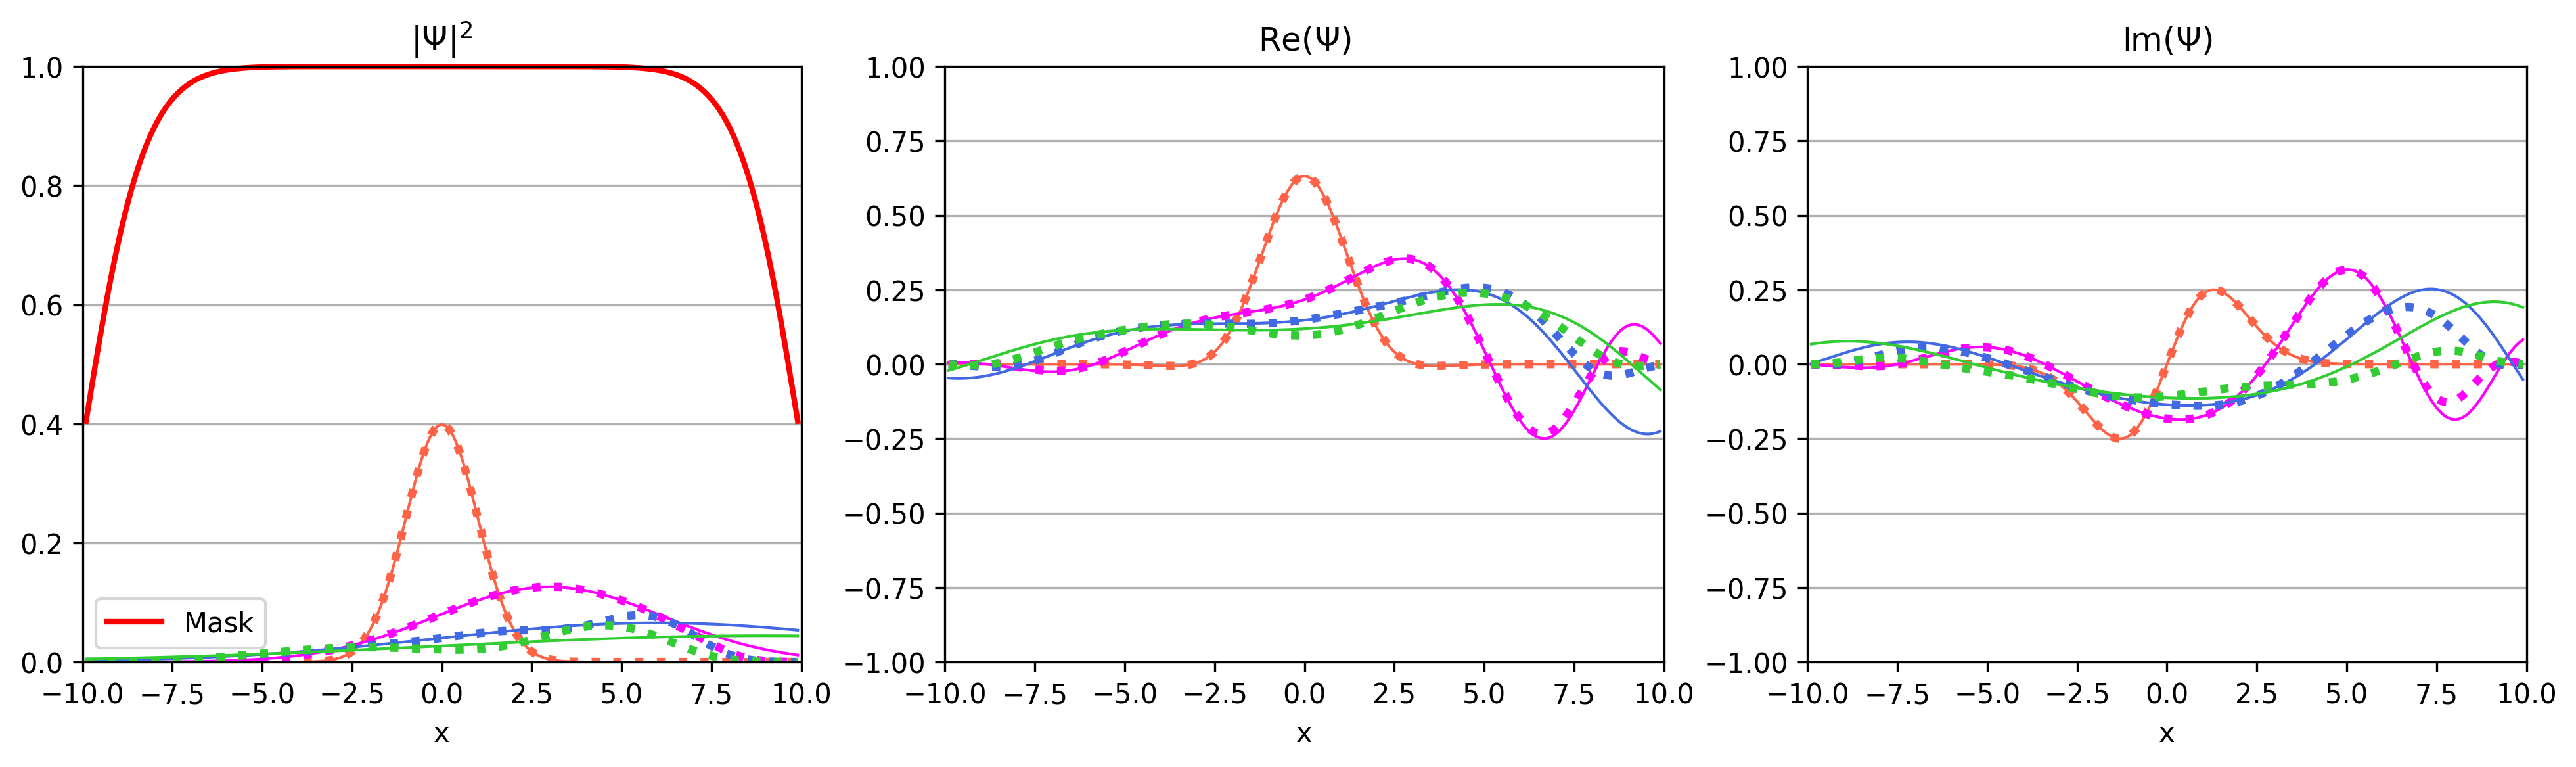
\includegraphics[width=\textwidth]{../figures/comparison.png}
 \caption{Сравнение численного и аналитических решений. Точки соответсвуют численному решению, а непрервная линия --- аналитическому. Красный цвет обозначает волновые функции при $t=0$, маджента --- при $t=0.3$, королевский голубой --- при $t=0.6$ и лаймовый зеленый --- при $t=0.9$. Шаг по времени $\Delta t = 0.1$, а импульс волновой функции $k_0 = 0.5$.}
 \label{fig:1}
\end{figure}



\end{document}
